\documentclass[a4paper,twoside,titlepage,12pt]{article}
%
% Suomalaiset asetukset
\usepackage[finnish]{babel}
\usepackage[utf8]{inputenc}
\parindent0.0cm
\parskip0.23cm % Toista \tableofcontents:n jälkeen, muuten tulee harva sisällysluettelo
\frenchspacing
%
% Muita paketteja
\usepackage{listings}
\lstloadlanguages{SQL,Python}
\renewcommand{\lstlistingname}{Listaus}
\renewcommand{\lstlistlistingname}{Listaukset}

\usepackage{tikz}
\usepackage{graphicx}

% European Computer Modern fonts, scalable Type1 instead of bitmap fonts
\usepackage{ae}

%\pagestyle{headings}

%
% Hyperref pitää ladata viimeisenä
\usepackage{hyperref}

\begin{document}


%
% Etusivu
%
\begin{titlepage}

\vskip5.0cm

\begin{center}

{\huge
\vspace*{0.0cm}
\parskip1.0cm
\emph{Minivr}: junayhtiön tietojärjestelmä

Kurssin T-76.1143 harjoitustyö

{ \Large 5.11.2010 }

{ \Large Ryhmä 55: }

\large
Mikko Markus Torni $<$mtorni@cc.hut.fi$>$ (51161R) \\
    Sami J. Lehtinen $<$sjl@iki.fi$>$ (44814P) \\
    Matti Niemenmaa $<$mniemenm@cc.hut.fi$>$ (77243K)

}

\vskip5.0em

\vfill

\begin{flushleft}

\emph{Lähdekoodi:}

\indent \url{https://github.com/sjlehtin/minivr/}

\emph{Käyttöliittymädemo:} \\
\url{http://semeai.org:8000/}

\emph{Toteutusalusta:} Python + Django, PostgreSQL 8.0+

\emph{Demoajankohta:} 11.11. klo 15:20

\end{flushleft}

\end{center}


\end{titlepage}

\newpage

%
% Ensimmäinen sivu, sisällysluettelo
%

\parskip0.00cm % Ilman tätä tulee harva sisällysluettelo

\tableofcontents
\listoffigures
\lstlistoflistings

\parskip0.23cm % Vasta \tableofcontents:n jälkeen, muuten tulee harva sisällysluettelo

\newpage

%
% Ensimmäinen varsinainen tekstisivu
%

\section{Johdanto}

Teimme \href{http://www.aalto.fi/}{Aalto-yliopiston} \href{http://www.tkk.fi/}{Teknilliseen korkeakoulun} tiedonhallintajärjestelmät-kurssille (T-76.1143) vuoden 2010 syyslukukaudella harjoitustyön.



\subsection{Tehtävänanto: junayhtiön tietojärjestelmä}

Valitsimme kurssin T-76.1143 annetuista harjoitustyöaiheista junayhtiön tietojärjestelmän. Tehtävä oli annettu seuraavasti:

\begin{quotation}
\itshape
Asiakkaat voivat hakea palvelun kautta juna-aikatauluja, ja varata lippuja (jotka ovat haettavissa asemalta lähdettäessä), mikäli niitä on jäljellä. Lippujen hinnat riippuvat pääteasemista, junavuorosta sekä ostajan statuksesta (opiskelija/aikuinen jne.). Eri junavuoroilla on omat lähtö -ja päätepysäkit, eivätkä junavuorot välttämättä pysähdy kaikilla asemilla. Reitit haarautuvat rautatieverkostossa täysin mielivaltaisesti. Esimerkiksi pysäkiltä B voi olla kiskot pysäkeille A, C, D ja E, eikä ainoastaan "edelliselle pysäkille A ja seuraavalle pysäkille C". Järjestelmän tulisi pystyä näyttämään käyttälle reittioppaan tavoin eri vaihtoehdot matkustaa paikasta x paikkaan y, huomioiden mahdolliset vaihdot, sekä optimoiden ajankäytön ja hinnan.

Junavuoron voi olettaa kulkevan eri kausina (kesä/talvi) tietyn viikonpäivän tiettyyn kellonaikaan. Eri junavuorojen nopeuksista toisiinsa nähden ei voi tehdä mitään oletuksia.

Aihe tarjoaa paljon haastetta ja päänvaivaa erityisesti tietokannan rakenteen suunnittelussa. Haastetta voi kasvattaa entisestään esimerkiksi muuttamalla osan junavuoroista lähijuniksi, jolloin lippuja ei voi varata ennalta, ja hinnoittelu tapahtuu kuljettujen vyöhykkeiden perusteella. Toisaalta kaukojunien liput voisi pystyä varaamaan tietylle istumapaikalle tiettyyn vaunuluokkaan (travel/business).

Aiheeseen voi ottaa ideoita esim. VR:n sivuita. 
\end{quotation}

\subsection{Järjestelmän vaatimukset}
\textbf{TODO:} Selvitys järjestelmän käyttötarkoituksesta ja sitä käyttävien käyttäjäryhmien tarpeista.

Käyttäjät etsivät järjestelmää käyttäen itselleen sopivia junavuoroja.
Järjestelmän pitää pystyä hakemaan käyttäjälle reitti annettujen asemien
välille, siten että jos suoraa yhteyttä ei löydy, järjestelmä yrittää
löytää käyttäjälle mahdollisimman hyvän reitin.  Käyttäjän pitää pystyä
varaamaan lippuja valitsemalleen reitille.

\section{Tietokanta}

Valitsimme toteutukseen vapaan PostgreSQL\footnote{\url{http://www.postgresql.org/}}-tietokannan. PostgreSQL on ohjelmistosuunnittelijaystävällinen sekä tarjoaa suorituskykyä ja joustavan indeksoinnin.

\subsection{ER-malli}

\begin{figure}
  \includegraphics[scale=0.5,angle=270]{relations}
  \caption{ER-malli keskeisimmista relaatioista}
\end{figure}

\textbf{TODO:} Kaavion sanallinen selvennys. Selittäkää ER-kaaviossa tehdyt ratkaisut, kaavion täytyy olla ulkopuolisen ymmärrettävissä. 

\subsubsection{Connection}
Kuvaa yhteyttä kahden aseman välillä.

\subsubsection{CustomerType}

Asiakastyyppi lipulle.  Pääasiassa alennuslippujen
määrittelyyn.

\subsubsection{Service}

Junavuoro.

\subsubsection{Station}

Asema, jolta junat lähtevät ja pysähtyvät.

\subsubsection{Stop}

Yksittäinen pysähdys asemalla.

\subsubsection{Ticket}

Vuorolle varattu lippu.

\subsubsection{Train}

Juna, jolla vuoro ajetaan.

\subsection{Tietokantataulut}

Taulujen luontikomennot ovat listauksessa~\ref{lst:sqlcreatetables} sivulla~\pageref{lst:sqlcreatetables}. Tietokantataulut luotiin Djangon objekti-relaatiokuvausmoduulia käyttäen, joka loi SQL-taulut ja päivitti tietokantarakenteet kehityksen aikana.

\begin{lstlisting}
CREATE TABLE minivr_junavuorot (ID TEXT PRIMARY KEY NOT NULL);
INSERT INTO minivr_junavuorot ('7652');
\end{lstlisting}

\subsubsection{Normalisointi}
\textbf{TODO:} Esitys funktionaalisista riippuvuuksista taulujen attribuuttien välillä. Ovatko taulut BCNF-normaalimuodossa? BCNF-normaalimuodon rikkominen edellyttää perustelut. 

\subsubsection{Indeksointi}
\textbf{TODO:} Käytetyn indeksoinnin perustelut.

\section{Käyttöliittymä}

Ryhmän jäsenten kiinnostuksen perusteella valitsimme käyttöliittymän toteutukseen \href{http://www.python.org/}{Pythonin}-ohjelmointikielen\footnote{\url{http://www.python.org/}} ja Python-pohjaisen \href{http://www.djangoproject.com/}{Django-kehitysrungon}\footnote{\url{http://www.djangoproject.com/}}.

Django on korkean tason Web-kehitysympäristö joka kannustaa nopeaan kehitykseen ja puhtaaseen, pragmaattiseen suunnitteluun. Djangon ominaisuuksista käytimme objekti-relaatiokuvausta, jonka avulla ohjelmoidessa ei tarvitse erikseen työstää SQL-rajapinnan tietotyyppimuunnoksia.

Ohjelmistokehityksen apuna käytimme Djangon mukana tulevaa kehityswebbipalvelinta joka soveltuu hyvin prototyyppivaiheeseen.

Tässä osassa esittelemme käyttöliittymän keskeisimmät sivut ja toiminnallisuudet.

\subsection{Yleistä}
Käyttäjä voi useimmissa ruuduissa klikata junavuoron nimeä jolloin näkyviin tulee asemakohtaiset aikataulut, tai käyttää \emph{Varaa}-painiketta paikan varaamiseen junavuoroon.

\subsection{Reitin haku}
Sivulla käyttäjä voi hakea vuoroja asemalta mille tahansa muulle asemalle. Käyttäjän täytyy syöttää toivottu lähtö- tai saapumisaika. Haun tuloksena käyttäjälle näytetään kaikki mahdolliset junavuorot saman vuorokauden sisällä.

Haun suorittamisen jälkeen käyttäjällä on mahdollisuus varata paikka junavuoroon painamalla \emph{Varaa}-painiketta. Järjestelmä ilmoittaa onnistuiko varaus.

\begin{figure}
  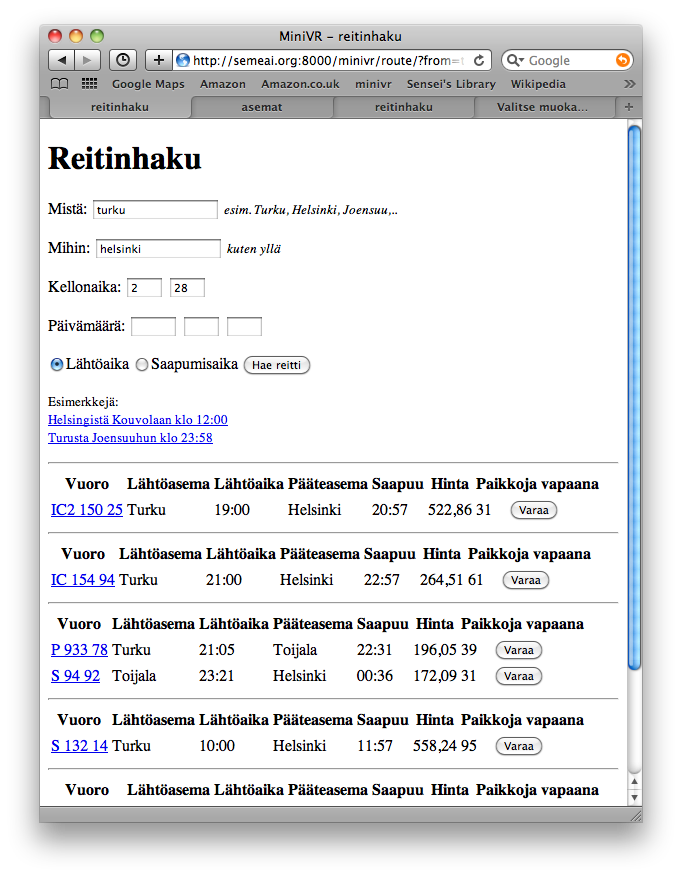
\includegraphics[width=100mm]{route.png}
  \caption{Reitinhaku}
\end{figure}

\subsection{Kaikki junavuorot}
Sivulla näkyy listaus kaikista junavuoroista lähtö- ja pääteasemineen.

\subsection{Varauksen onnistuminen}

Reittihausta varauksen onnistuminen (tai epäonnistuminen) näytetään
käyttäjälle erillisellä sivulla.

Tältä sivulta pitäisi pystyä palaamaan rettihakusivulle (tämä on vielä
tekemättä).

\subsection{Käyttöliittymäsivu \ldots}
\textbf{TODO:} Käyttöliittymäsivujen esittely sivu kerrallaan, siten että jokaisen sivun käyttötarkoitus ilmenee. Kertokaa käyttäjän syöttämien tietojen tarkistuksesta. Screenshotit ovat hyvä juttu. 

\section{Viimeistely}

Ryhmällä on tarkoitus vielä lisätä lisätä linkkejä sivujen välille
käyttökokemuksen parantamiseksi (mm. varauksen vahvistussivulta takaisin
reittihakuun).

Virhesivuja ei ole viimeistelty (kaksi yhtäaikaista varausta viimeiseen
paikkaan, toinen siis epäonnistuu).

\section{Loppusanat}
\subsection{Työmäärä}
\textbf{TODO:} Lisäksi toivomme myös rehellistä selvitystä töiden jakautumisesta ryhmän jäsenten kesken, sekä arvioita tehdyistä tunneista kunkin aktiviteetin osalta. Mikäli ette ole pitäneet tunneista kirjaa, summittaisetkin arviot kelpaavat. Tämän kappaleen tiedot eivät vaikuta työn arvosteluun.

Mikko Markus Torni käytti harjoitustyöhön aikaa yhden tunnin ideoiden ylös kirjaamiseen, 12 tuntia dokumentoinnissa, kaksi tuntia koodiin tutustumiseen.

\subsection{Oma arvio harjoitustyöstä}

Ryhmä aloitti työn tekemisen toden teolla aivan liian myöhään.

\subsection{Palaute kurssin järjestäjille}

Ei valittamista kurssijärjestelyistä.

%
% Liitteet
%
% 
\newpage
\section*{Tietokannan luontikomennot}

\lstinputlisting[language=SQL,breaklines=true,breakatwhitespace=true,frame=single,basicstyle=\small,label=lst:sqlcreatetables,caption=Tietokantataulujen luontikomennot]{minivr.sql}

\end{document}
